\section{IT Digital E07 - Instrução de Trabalho Digital (item 2e)}

\subsection{Função}

A IT Digital substitui a instrução impressa do posto E07 (Montagem de Tubulação) por uma página web (\cod{/instrucao/e07}) que avança sozinha, sincronizada com o ciclo real do posto 07 no CLP. São cinco telas: a capa (finalidade, condições de início e referência de ciclo) e quatro passos, cada um com a ação do operador, o que conferir antes de avançar e o que fazer se houver desvio (Tabela \ref{tab:itpassos}). A página recebe o estado a cada 100 ms pelo WebSocket \cod{/ws/instruction/e07} e o rodapé mostra o slide, a mensagem de sincronização e o tempo decorrido do ciclo (0 a 36 s).

{\footnotesize
\begin{longtable}{|>{\centering\arraybackslash}p{1.3cm}|>{\raggedright\arraybackslash}p{5.0cm}|>{\centering\arraybackslash}p{3.4cm}|>{\centering\arraybackslash}p{3.6cm}|}
\caption{Sequência da IT Digital E07 (\cod{domain/work\_instruction.py}: \cod{STEP\_ENDS = (7, 14, 29, 36)}).}\label{tab:itpassos}\\
\hline
\textbf{Slide} & \textbf{Conteúdo} & \textbf{Intervalo do ciclo} & \textbf{Duração} \\ \hline
\endfirsthead
\hline
\textbf{Slide} & \textbf{Conteúdo} & \textbf{Intervalo do ciclo} & \textbf{Duração} \\ \hline
\endhead
1 & Capa & fora do ciclo & - \\ \hline
2 & 01 Conferir unidade e kit & 0 a 7 s & 7 s \\ \hline
3 & 02 Posicionar no gabarito & 7 a 14 s & 7 s \\ \hline
4 & 03 Fixar as conexões & 14 a 29 s & 15 s \\ \hline
5 & 04 Inspecionar e registrar & 29 a 36 s & 7 s \\ \hline
\end{longtable}
}

\subsection{Regras de sincronização}

A lógica está em \cod{services/plc\_work\_instruction.py} e usa o relógio monotônico do receptor:

\begin{itemize}
    \item O ciclo começa quando \cod{D01657} (estado do P07, nó \cod{Linha/StatusProcesso}) \textbf{muda} para 2. Uma primeira leitura já em 2 não indica quando o ciclo começou; por isso, se o receptor se conectar com o posto processando, a tela espera o próximo ciclo.
    \item A instrução volta à capa quando o P07 sai do estado 2 (ciclo concluído) ou quando a sequência atinge 36 s. Se o P07 concluir antes de 36 s, a tela avisa que o ciclo foi mais curto que a sequência completa.
    \item Um Andon em qualquer posto coloca a instrução em \textbf{Linha parada} (capa, com o posto e a categoria). Liberado o Andon, o ciclo em curso não é retomado: a tela fica em \textbf{Aguardando próximo ciclo} até uma nova entrada do P07 no estado 2.
    \item Sem OPC UA, a tela mostra \textbf{Sem sincronização} e permanece na capa.
\end{itemize}

\subsection{Evidência: sincronização com o P07}

Na segunda execução da demonstração (Gateway real e CLP emulado, seção \ref{sec:emulado}), o estado da IT foi lido de \cod{/api/instruction/e07} e o do P07 de \cod{/api/snapshot} a cada $\sim$1,1 s (mediana), e a página foi capturada a cada mudança de slide (Figuras \ref{fig:it1} a \ref{fig:itsync}). A Tabela \ref{tab:itobs} compara as transições observadas com as esperadas.

{\footnotesize
\begin{longtable}{|>{\centering\arraybackslash}p{2.0cm}|>{\centering\arraybackslash}p{2.0cm}|>{\raggedright\arraybackslash}p{4.6cm}|>{\centering\arraybackslash}p{2.6cm}|>{\centering\arraybackslash}p{2.6cm}|}
\caption{Transições observadas da IT Digital (ciclo \cod{plc-p07-1} e seguintes). Tempos em segundos desde o Start; ``no ciclo'' é o \cod{elapsed\_seconds} informado pela API.}\label{tab:itobs}\\
\hline
\textbf{Instante (s)} & \textbf{D01657} & \textbf{Estado da IT} & \textbf{No ciclo (s)} & \textbf{Esperado (s)} \\ \hline
\endfirsthead
\hline
\textbf{Instante (s)} & \textbf{D01657} & \textbf{Estado da IT} & \textbf{No ciclo (s)} & \textbf{Esperado (s)} \\ \hline
\endhead
0,7 & 0 & aguardando, capa & - & - \\ \hline
64,2 & 1 $\rightarrow$ 2 & em ciclo, slide 2 & 0,4 & 0 \\ \hline
71,8 & 2 & em ciclo, slide 3 & 7,9 & 7 \\ \hline
78,1 & 2 & em ciclo, slide 4 & 14,1 & 14 \\ \hline
93,6 & 2 & em ciclo, slide 5 & 29,7 & 29 \\ \hline
100,9 & 2 $\rightarrow$ 1 (estado 3 não amostrado) & concluído, capa & 36,0 & 36 \\ \hline
104,7 & 2 & em ciclo (\cod{plc-p07-2}), slide 2 & 2,7 & - \\ \hline
114,0 & 2 & \textbf{linha parada} (Andon de Processo no P07) & - & - \\ \hline
124,0 & 2 & aguardando próximo ciclo (Andon liberado) & - & - \\ \hline
150,2 & 1 $\rightarrow$ 2 & em ciclo (\cod{plc-p07-3}), slide 2 & 0,5 & 0 \\ \hline
\end{longtable}
}

As trocas de slide ocorreram entre 0,1 e 0,9 s depois do limite teórico, diferença compatível com o intervalo de amostragem do teste ($\sim$1,1 s) somado ao ciclo de leitura do Gateway (250 ms). A instrução já aparecia interrompida na amostra seguinte ao Andon (intervalo de 1,3 s) e, após a liberação, a tela não retomou o ciclo interrompido, aguardando o ciclo seguinte (\cod{plc-p07-3}), como especificado.

\begin{figure}[H]
    \centering
    \begin{minipage}{0.49\textwidth}\centering
        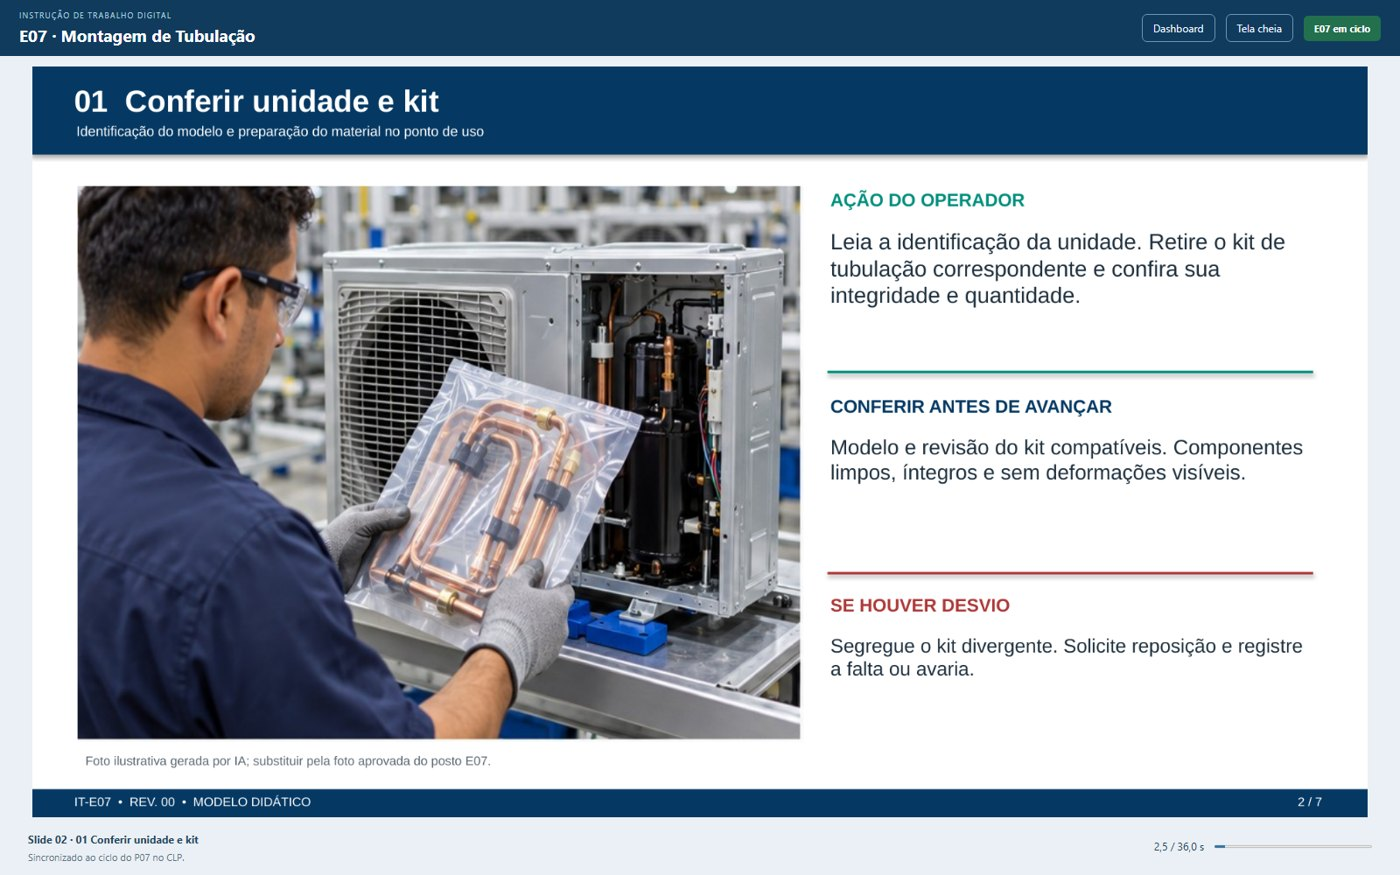
\includegraphics[width=\textwidth]{Imagens/it_running_slide2.jpg}
    \end{minipage}\hfill
    \begin{minipage}{0.49\textwidth}\centering
        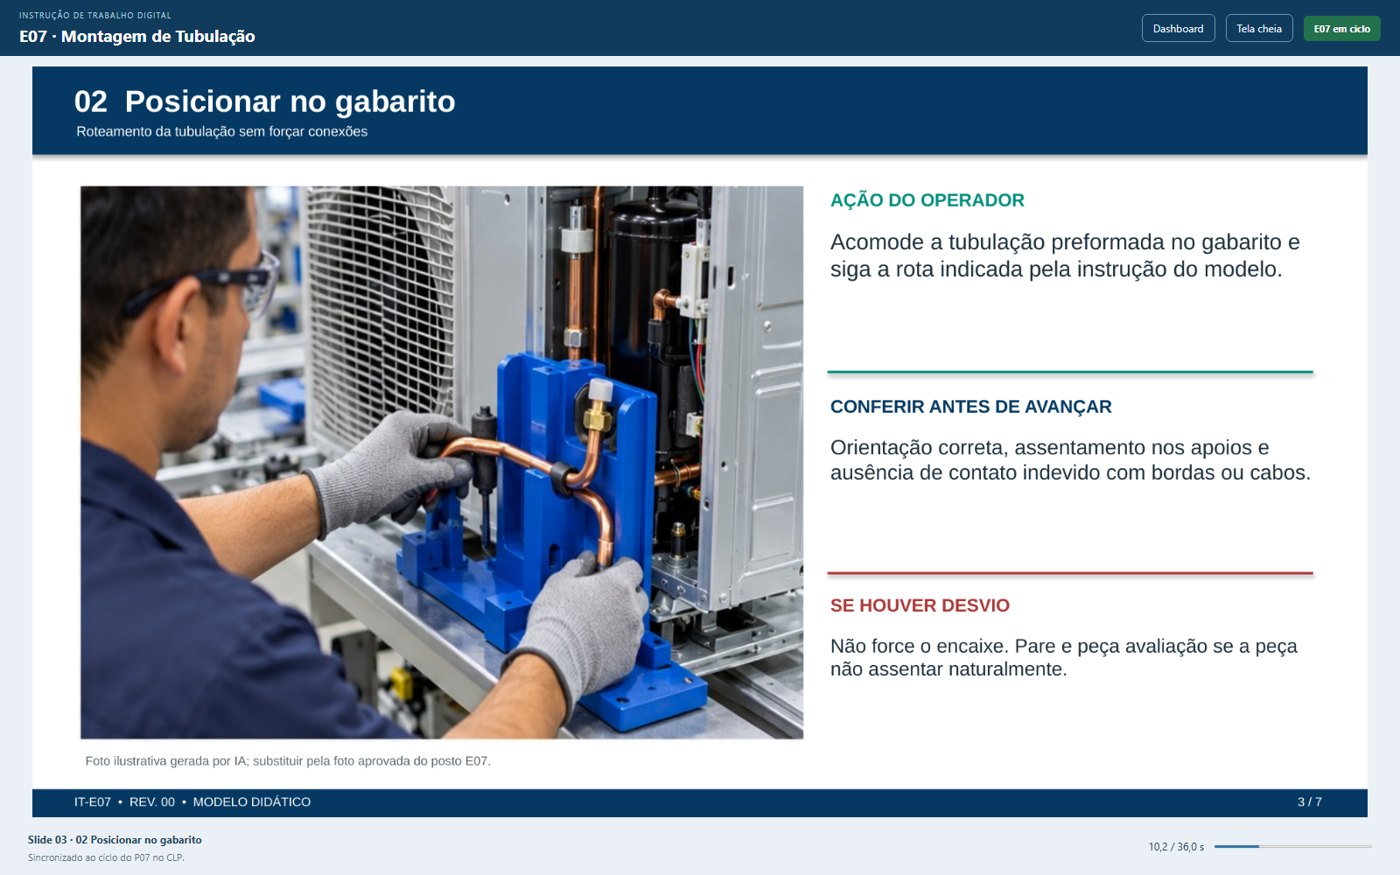
\includegraphics[width=\textwidth]{Imagens/it_running_slide3.jpg}
    \end{minipage}\\[0.2cm]
    \begin{minipage}{0.49\textwidth}\centering
        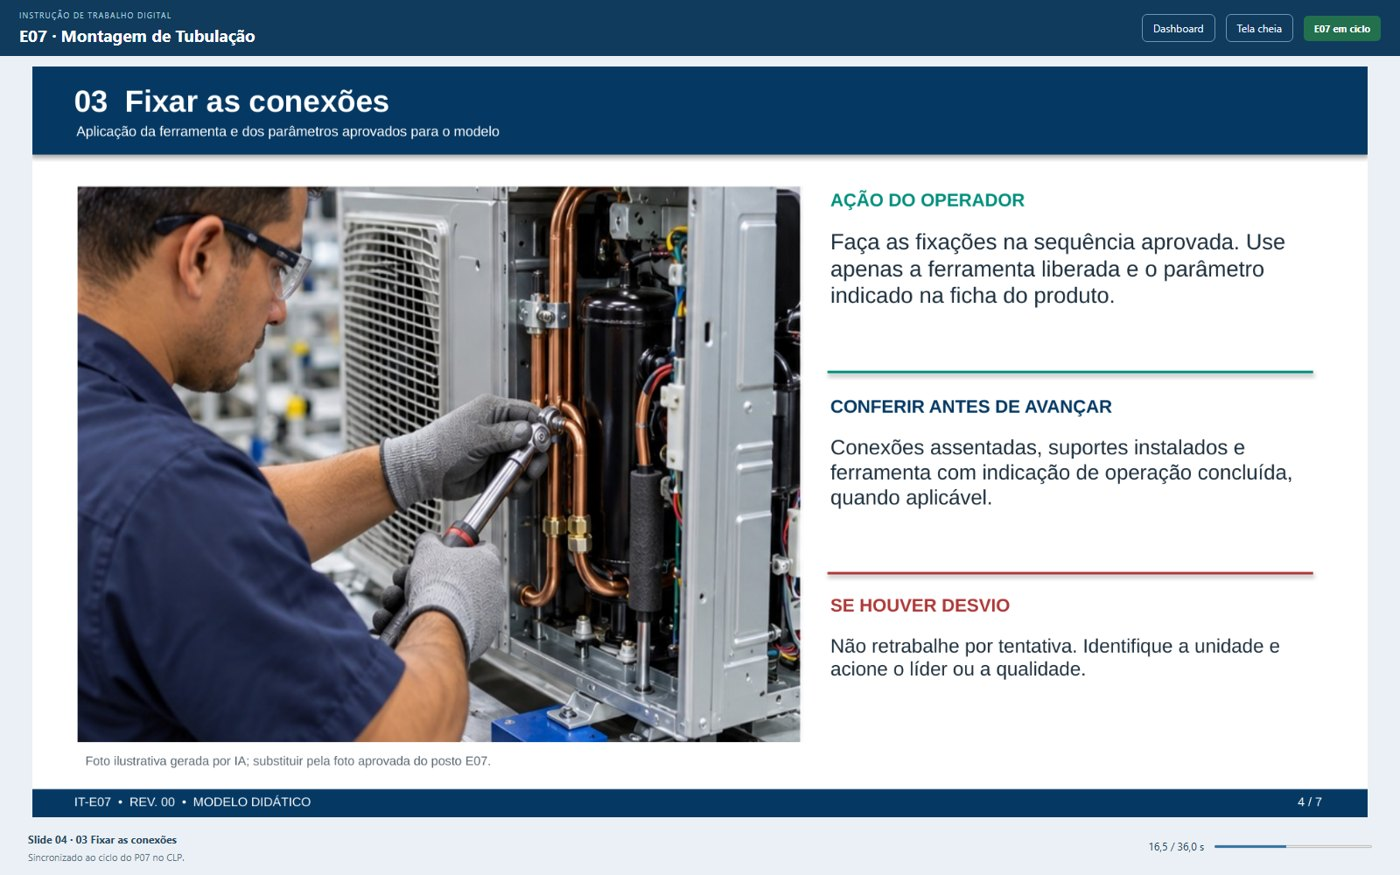
\includegraphics[width=\textwidth]{Imagens/it_running_slide4.jpg}
    \end{minipage}\hfill
    \begin{minipage}{0.49\textwidth}\centering
        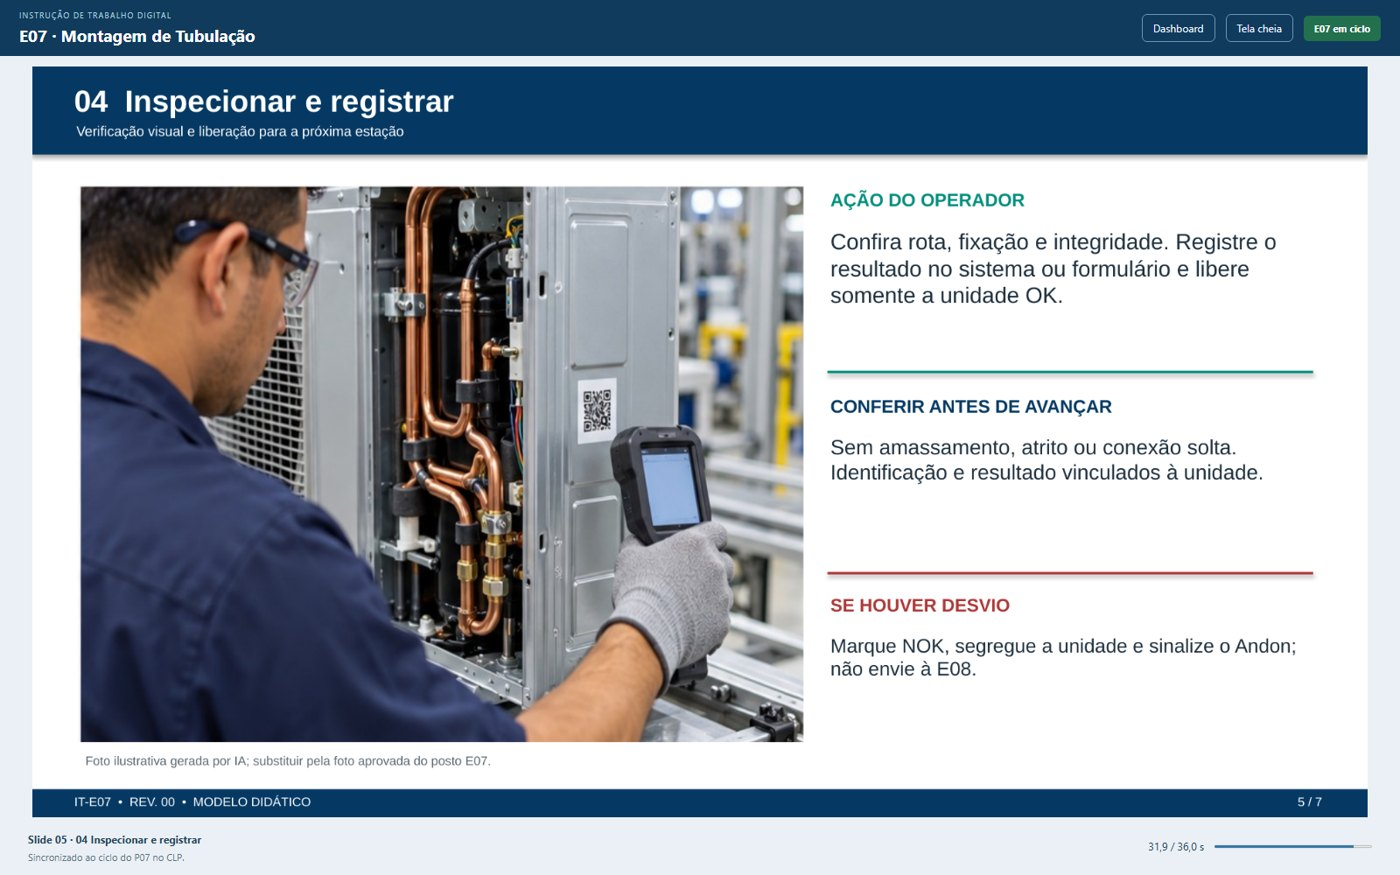
\includegraphics[width=\textwidth]{Imagens/it_running_slide5.jpg}
    \end{minipage}
    \caption{IT Digital durante o ciclo \cod{plc-p07-1}: passos 01 a 04 (slides 2 a 5), com ``E07 em ciclo'' e ``Sincronizado ao ciclo do P07 no CLP''. (arquivos: Imagens/it\_running\_slide2.jpg a it\_running\_slide5.jpg)}
    \label{fig:it1}
\end{figure}

\begin{figure}[H]
    \centering
    \begin{minipage}{0.49\textwidth}\centering
        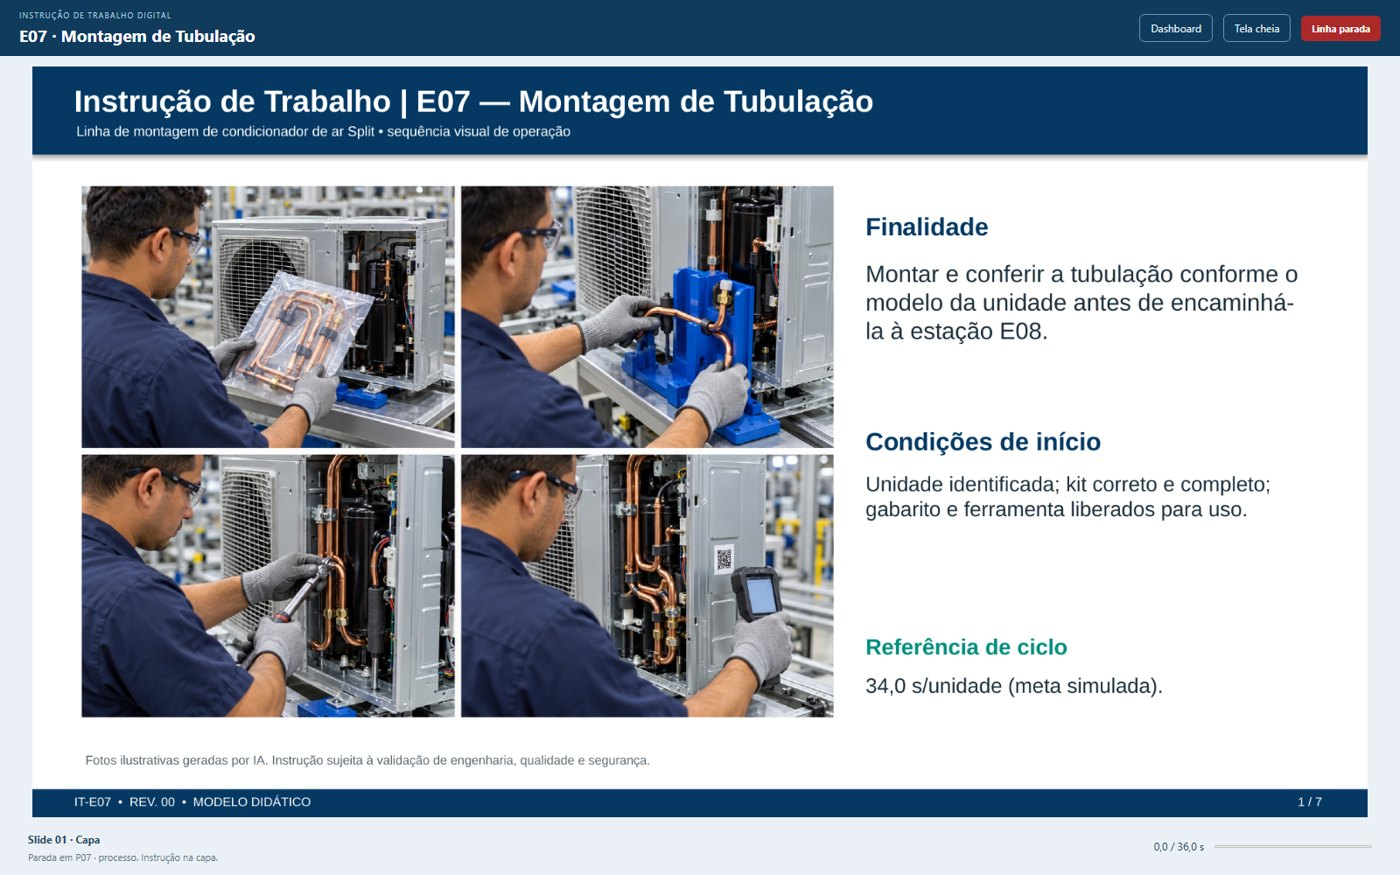
\includegraphics[width=\textwidth]{Imagens/it_paused_slide1.jpg}
    \end{minipage}\hfill
    \begin{minipage}{0.49\textwidth}\centering
        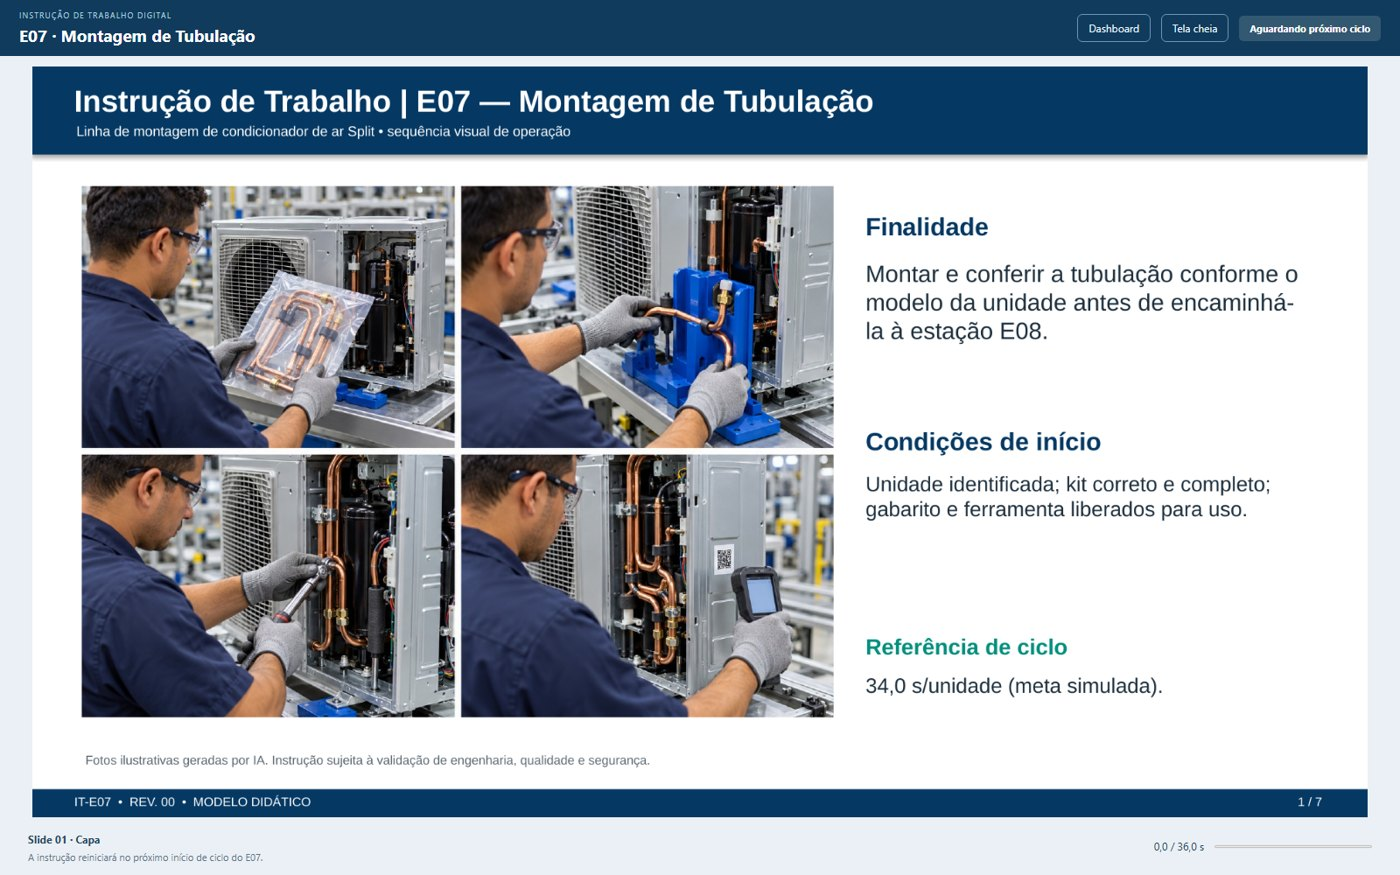
\includegraphics[width=\textwidth]{Imagens/it_interrupted_slide1.jpg}
    \end{minipage}
    \caption{Esquerda: Andon de Processo no P07 - ``Linha parada'', instrução na capa. Direita: após a liberação - ``Aguardando próximo ciclo''. (arquivos: Imagens/it\_paused\_slide1.jpg e it\_interrupted\_slide1.jpg)}
    \label{fig:it2}
\end{figure}

\begin{figure}[H]
    \centering
    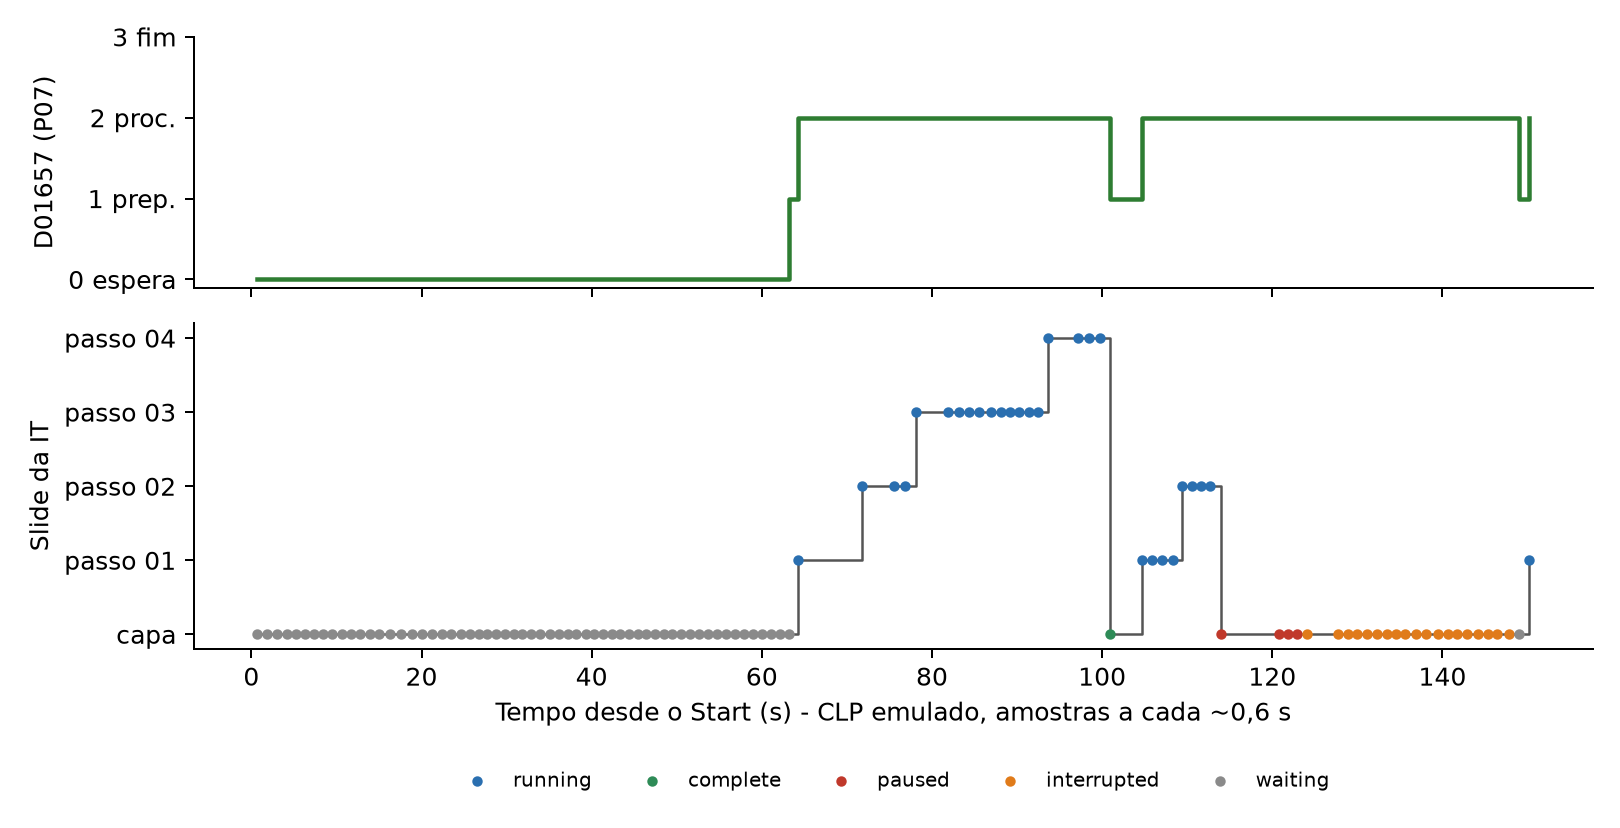
\includegraphics[width=1.00\textwidth]{Imagens/it_sincronizacao_p07.png}
    \caption{Estado do P07 (\cod{D01657}) e slide exibido pela IT Digital ao longo da demonstração. O intervalo mediano entre amostras foi de 1,1 s; o rótulo do eixo traz o valor nominal de 0,6 s. (arquivo: Imagens/it\_sincronizacao\_p07.png)}
    \label{fig:itsync}
\end{figure}

Os quatro testes de \cod{tests/test\_work\_instruction.py} verificam as mesmas regras sem o navegador: a sequência de 36 s, a interrupção por Andon até o próximo início, o descarte de estado inválido e a espera por um ciclo novo após reconexão.
